\subsection{Preliminaries}

\subsubsection{Bridge}
A \emph{bridge} is an interoperability protocol between two ledger protocols.
The purpose of the bridge is to relay events or information that take place on
the source side to the destination side. In particular, the parties that
maintain the bridge transmit \emph{cross-chain} transactions, such that a
transaction on the source side is represented by an ``image'' on the
destination side.

There are two core properties that a secure bridge should guarantee: safety and
liveness.

\paragraph{Bridge Safety.}
Bridge safety mandates that a transaction appears on the destination side \emph{only if} it has first
appeared on the source side, albeit with some delay.
%
Intuitively, safety ensures that \emph{bad
things don't happen}, that is it's impossible to find a transaction paying out on the
destination without its ``pre-image'' having appeared on the source side. 
In essence, if safety is guaranteed, an adversary cannot create money on the
destination side without having paid on the source side.
%
Figure~\ref{fig:bridge-safety} illustrates bridge safety.
The party $P_2$ first observes the transaction image $\tx$ on the destination
side ($\Pi_2$) at time $r_1$, and expects another party $P_1$ to have already
seen the transaction's pre-image $\phi^{-1}(\tx)$ on the source side ($\Pi_1$).
Note that, due to network and consensus delays, this may be observed with a
(bounded) delay.

\begin{figure}
    \center
    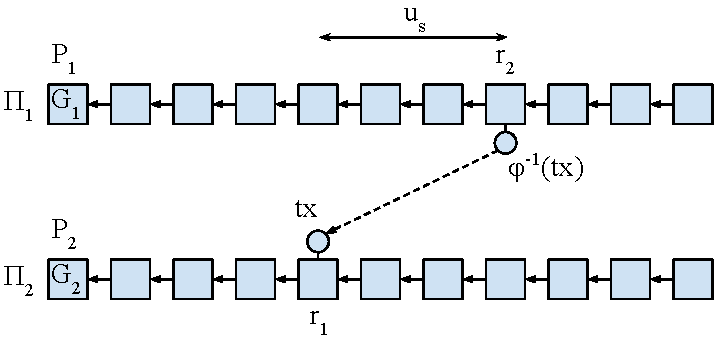
\includegraphics[width=0.8\columnwidth]{figures/bridge-safety.pdf}
    \caption{Bridge safety}
    \label{fig:bridge-safety}
\end{figure}

\paragraph{Bridge Liveness.}
Bridge liveness ensures that a transaction which appears on the source side will eventually make
it to the destination side. Intuitively, this guarantees that \emph{good things happen}, that is whenever an
honest party attempts to cross the bridge, it will successfully do so.
A visual depiction of bridge liveness is shown in Figure~\ref{fig:bridge-liveness}.
% Even though our treatment is general to all ledger protocols and not particular to blockchains,
% here we illustrate a blockchain example. 
A block containing transaction $\tx$ appears in the source side ($\Pi_1$) in the view
of a party $P_1$ at time $r_1$. Soon after, in round $r_2 \leq r_1 + u\ell$, the corresponding transaction image
$\phi(\tx)$ appears in the view of another party $P_2$ on the destination side ($\Pi_2$).

\begin{figure}
    \center
    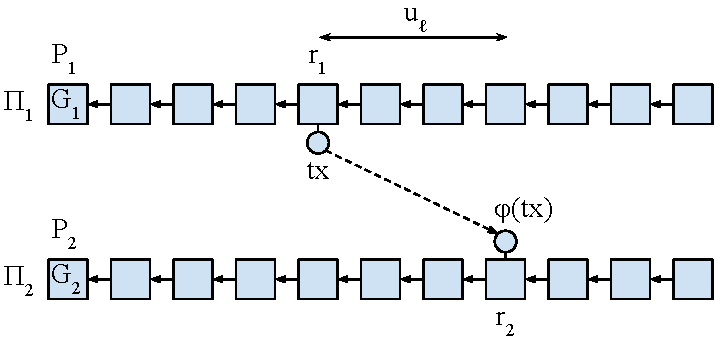
\includegraphics[width=0.7\columnwidth]{figures/bridge-liveness.pdf}
    \caption{Bridge liveness}
    \label{fig:bridge-liveness}
\end{figure}

\subsubsection{Light Clients}

A \emph{light client} is a client that wishes to synchronize with the rest
of the network, but has limited resources available in terms of communication,
computation, and storage. One example of a limited resource computer is the
on-chain smart contract infrastructure of Axelar, where computation and storage
are expensive. The light client begins its lifecycle holding the genesis block
and synchronizes to the current tip of the canonical chain once in a while.
Our job when building a light client is, given a block that the light client
has already downloaded sometime in the past, to allow the client to
synchronize with the most recent chain tip.

% TODO(shresth): Add a separate section before this to describe
% the high-level architecture of the on-chain light client without
% discussing the particularities of the Ethereum sync committee.
% Concretely, talk about how the data moves from Ethereum to
% Axelar when validators are dishonest and how they can be caught.

% TODO(shresth): Add a figure here.

\subsubsection{Ethereum Sync Committee}\label{subsec:sync-committee}

One useful ingredient of the Ethereum ecosystem that enables the
construction of efficient light clients is the so-called \emph{sync committee}~\cite{sync-committee}.
This feature was introduced in the system's
``Altair'' hard fork and is specifically tailored for use of light clients, as
we will discuss in the alternatives of Section~\ref{subsec:alternatives}.

The sync committee consists of $512$ of Ethereum validators. They are randomly
selected, from the set of all validators, every sync committee period (approx.
$1$ day). Each honest validator in the sync committee is continually online and
signs the header of each block that is added to the chain's tip on every slot. 

The sync committee of period $X$ is decided two periods before it takes effect,
that is during period $X-1$. The root of the Merkle tree that defines the
committee is published in the header of each block in the immediate period
before it is activated, that is in period $X-1$, along with the root of that
($X-1$) period's active committee. Consequently, when a block is validated in
this period, the committee is authorized to take effect at the beginning of its
designated period. Crucially, the existence of a block, which contains (in its
header) the roots of both the active and the following committee can serve as
proof of the ``handover'' from one committee to the other. Note that a block is
validated if it is signed by at least $\frac{2}{3}$ of all committee members.

We demonstrate the usage of the sync committee with the following example.
Assume that a client $C$ holds the block header of some slot $N$, that is part
of the sync committee period $X$.  When $C$ wants to authenticate the header of
a block at slot $N'$, which is part of the period $X+1$, it proceeds as
follows.  First, $C$ validates the sync committee of period $X+1$. To do so, it
verifies that the Merkle root of the committee was published in a block header
of period $X$; if so, $C$ updates its sync committee for $X+1$ as the one
defined in the Merkle tree. At this point, $C$ can validate every block header
for each slot of period $X+1$, by obtaining the corresponding signatures of the
sync committee of that period.

Using this iterative process, the light client can validate all future blocks,
starting from an initial trusted point. The cost of validating a block depends
on the size of the committee, the aggregate signature, and the Merkle path; in
Ethereum this is estimated to approx. $25$KB~\cite{sync-committee}.

There are two main points of discussion around the sync committee.
%
First, the committee should be honest. In essence, the sampling process, via
which the sync committee's members are chosen from the set of all Ethereum
validators, should be secure, s.t. the probability that $\frac{2}{3}$ of the
committee members are adversarial is negligible. Observe that, if the committee
is malicious, then it can convince a light client of a fraudulent Ethereum
state. 
%
Second, slashing is currently not implemented in the sync committee. Therefore,
a committee member can double-sign, i.e., sign conflicting blocks, without
direct counterincentives. Whether committee members are incentivized to behave
in such manner is outside the scope of this document, although it is an
interesting research question.
